
\subsection{Contributions and Spatial Effects of Regional Aerodynamic Knowledge}
\label{sec:regional_knowledge_contributions}

The contribution of transferred aerodynamic knowledge is not uniform along the wing span. Figure~\ref{fig:vb_spanwise} compares the sectional pressure-prediction errors of M0, M1, and M2 at three target-domain training sizes. Relative to direct three-dimensional learning (M0), sectional knowledge transfer (M1) reduces the errors over a broad spanwise range, whereas the additional gains from regional knowledge (M2) vary with spanwise position. The differences are particularly evident at $N=10$ and $20$, for which M2 yields lower mean sectional RMSE than M1 throughout the evaluated span on both surfaces. At $N=100$, the errors are considerably smaller and the two knowledge-based models approach one another, with limited local reversals in their relative performance. The larger upper-surface errors, especially toward the outboard wing, also indicate that the remaining prediction difficulty is spatially nonuniform. Thus, the additional value of regional knowledge depends on both spanwise location and the amount of target-domain supervision.

\begin{figure*}[t]
    \centering
    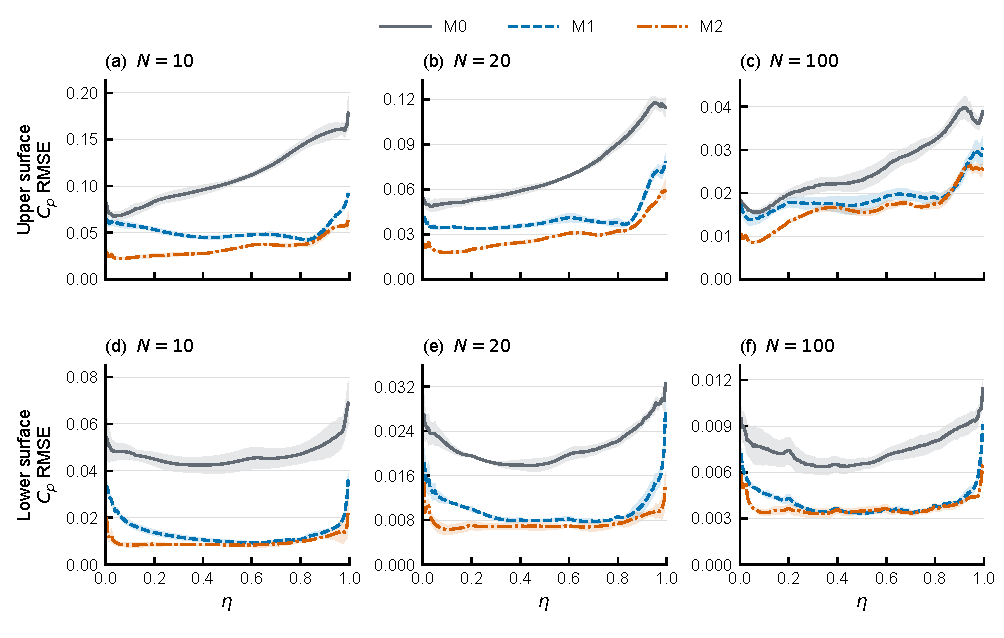
\includegraphics[width=\textwidth]{V_Results_and_Discussion/figures/V_B_Fig14/V_B_Fig14_vb_spanwise.pdf}
    \caption{Spanwise sectional RMSE of M0, M1, and M2 at three training sizes for both surfaces (88 test wings; mean $\pm$ standard deviation over three runs).}
    \label{fig:vb_spanwise}
\end{figure*}



The ablation results at $N=20$ clarify the distinct spatial contributions of the two regional knowledge components (Fig.~\ref{fig:vb_ablation}). Relative to M1, retaining only the wing-root correction (AR) reduces the root-region RMSE by $36.25\%$, but provides a much smaller improvement near the tip. In contrast, retaining only the wing-tip correction (AT) reduces the tip-region RMSE by $17.81\%$, while increasing the root-region error by $5.47\%$. These contrasting responses are consistent with the different spatial characteristics represented by the root and tip knowledge models. When both components are included, M2 attains the lowest mean RMSE among the four configurations in all three regions, with reductions of $39.81\%$, $24.69\%$, and $20.66\%$ relative to M1 in the root, midspan, and tip regions, respectively. The improvement in the midspan region indicates that the benefits of regional knowledge are not confined to the regions used to define the corrections. Nevertheless, the additional gain of M2 over the corresponding single-region model is comparatively modest, particularly near the tip, and is not reproduced in every training run. The combined prior therefore improves the regional averages without ensuring a uniform advantage at every location.

\begin{figure*}[t]
    \centering
    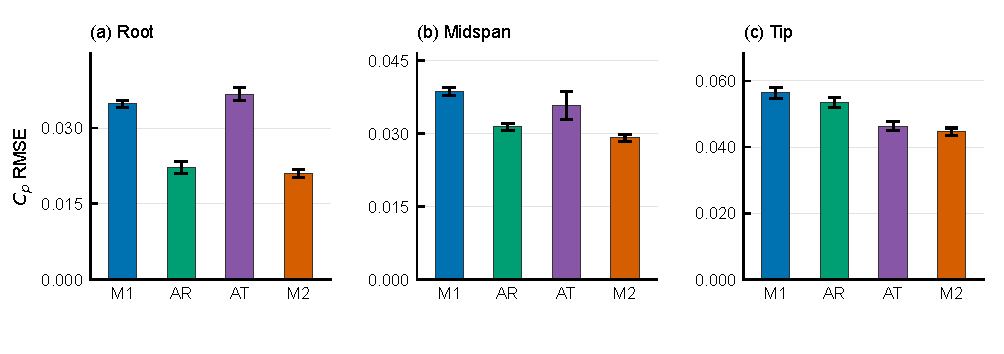
\includegraphics[width=\textwidth]{V_Results_and_Discussion/figures/V_B_Fig15/V_B_Fig15_vb_ablation.pdf}
    \caption{Regional pressure RMSE at $N=20$: (a) root, (b) midspan, and (c) tip.}
    \label{fig:vb_ablation}
\end{figure*}

The reconstruction of the chordwise pressure distributions provides a complementary view of these error statistics. Figure~\ref{fig:vb_cp_sections} shows ten spanwise sections of a test wing at $M_\infty=0.7836$ and $\alpha=3.512^\circ$, predicted by M2 at $N=20$. When the 88 test wings were ranked in ascending order of whole-wing $C_p$ RMSE averaged over the three M2 training runs, this wing ranked 54th. Across the span, M2 reproduces the main upper- and lower-surface pressure trends, including the suction distributions and subsequent pressure recovery. Agreement is closer at $\eta\approx0.755$ and $0.850$, whereas appreciable upper-surface discrepancies remain around $\eta\approx0.550$ and $0.655$. The combined sectional RMSE ranges from $0.01483$ to $0.04209$ among the ten displayed sections. The resulting variation shows that an accurate overall pressure reconstruction can coexist with localized errors in the chordwise loading distribution.

\begin{figure*}[t]
    \centering
    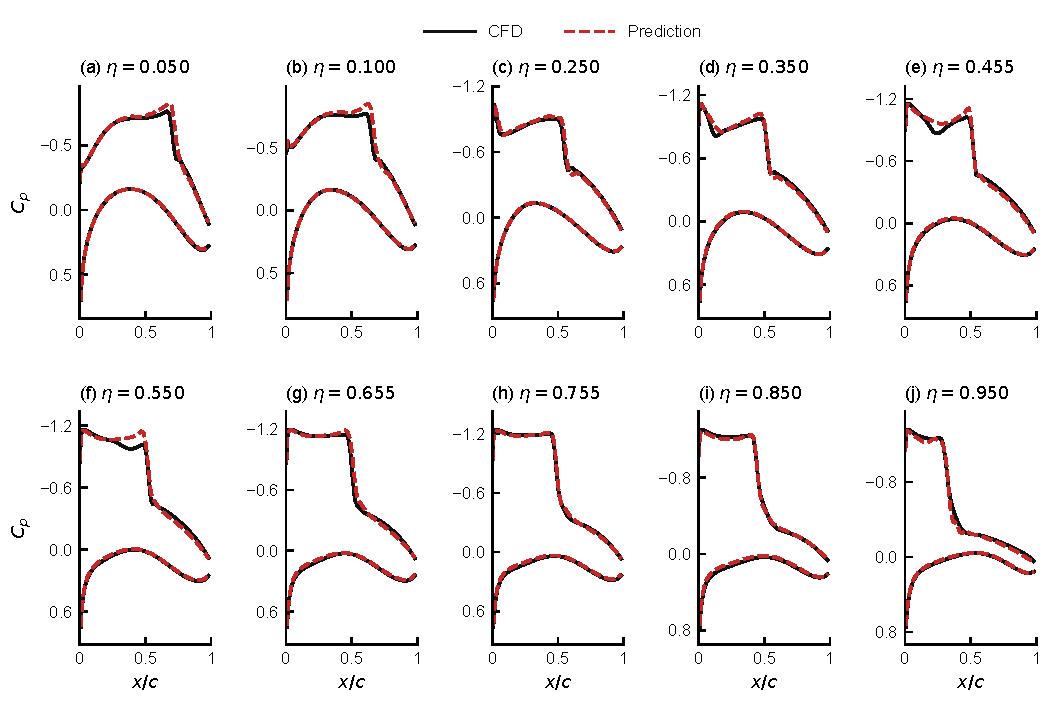
\includegraphics[width=\textwidth]{V_Results_and_Discussion/figures/V_B_Fig16/V_B_Fig16_vb_cp_sections.pdf}
    \caption{CFD and M2 pressure distributions at ten spanwise sections ($M_\infty=0.7836$, $\alpha=3.512^\circ$; $N=20$).}
    \label{fig:vb_cp_sections}
\end{figure*}

For the same test wing shown in Fig.~\ref{fig:vb_cp_sections}, the local pressure comparisons in Fig.~\ref{fig:vb_cp_regions} further show why regional-average improvements should not be interpreted as gains at every section. At the root section ($\eta\approx0.100$), AR reduces the lower-surface RMSE from $0.01151$ for M1 to $0.00343$, while the upper-surface RMSE increases slightly because of residual discrepancies in the aft-chord pressure recovery. Consequently, the combined sectional RMSE changes only marginally; M2 exhibits a larger upper-surface error at this particular section. A similar surface-dependent response occurs at the tip section ($\eta\approx0.950$). AT lowers the lower-surface RMSE from $0.01321$ to $0.00393$, but its upper-surface error increases, resulting in a higher combined sectional RMSE than M1. These case-specific deviations do not contradict the improvements observed over the 88-wing test set. Rather, they illustrate that regional knowledge contributes useful finite-wing pressure information whose effectiveness depends on the local pressure characteristics and its interaction with target-domain residual learning. Further improvement of the hierarchical framework therefore requires not only transferable regional corrections but also their appropriate combination across the wing surface.

\begin{figure*}[t]
    \centering
    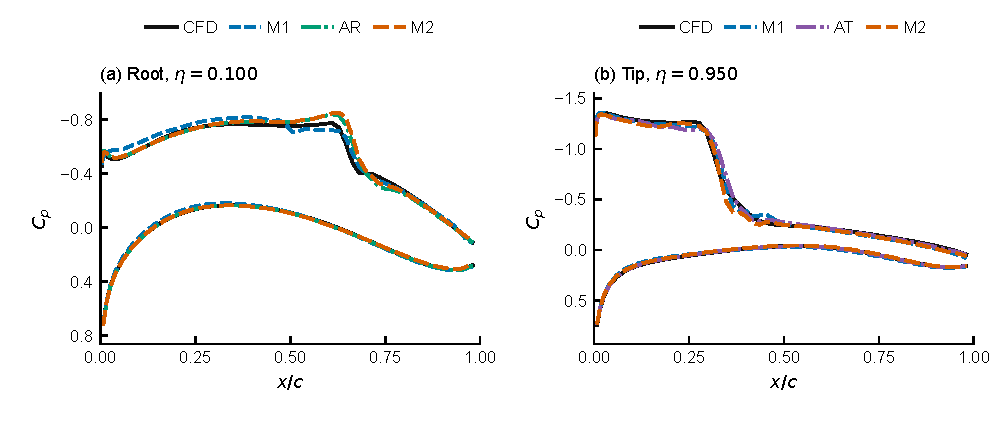
\includegraphics[width=\textwidth]{V_Results_and_Discussion/figures/V_B_Fig17/V_B_Fig17_vb_cp_regions.pdf}
    \caption{Local pressure distributions at the near-root ($\eta\approx0.100$) and near-tip ($\eta\approx0.950$) sections of the test wing in Fig.~\ref{fig:vb_cp_sections} ($N=20$).}
    \label{fig:vb_cp_regions}
\end{figure*}
